\documentclass[11pt]{article}

\usepackage{latexsym}
\usepackage{graphicx}
\usepackage{amssymb}
\usepackage{amsthm}
\usepackage{enumerate}
\usepackage{amsmath}
\usepackage{cancel}
\numberwithin{equation}{section}
\numberwithin{figure}{section}
\numberwithin{table}{section}

\setlength{\evensidemargin}{.25in}
\setlength{\oddsidemargin}{-.25in}
\setlength{\topmargin}{-.75in}
\setlength{\textwidth}{6.5in}
\setlength{\textheight}{9.5in}
\newcommand{\due}{February 24th, 2010}
\newcommand{\HWnum}{4}
\newcommand{\grad}{\bold\nabla}
\newcommand{\vecE}{\vec{E}}
\newcommand{\scrptR}{\vec{\mathfrak{R}}}
\newcommand{\kapa}{\frac{1}{4\pi\epsilon_0}}
\newcommand{\unit}[1]{\ensuremath{\, \mathrm{#1}}}

\begin{document}
\begin{titlepage}
\setlength{\topmargin}{1.5in}
\begin{center}
\Huge{Physics 3320} \\
\LARGE{Principles of Electricity and Magnetism II} \\
\Large{Professor Ana Maria Rey} \\[1cm]

\huge{Homework \#\HWnum}\\[0.5cm]

\large{Joe Becker} \\
\large{SID: 810-07-1484} \\
\large{\due} 

\end{center}

\end{titlepage}



\section{Introduction}
By using positive feedback in an operational amplifier we increase the gain of the op-amp. But this comes at a cost, spontaneous oscillations in the output voltage can occur due to internal capacitance or inductance in the coaxial cables. This lab will use a LC filter in the positive feedback loop to test the effects of capacitance and inductance on the op-amp.

\section{Theory}
Basic op-amp properties that we are assuming is that the output voltage is given by
\begin{equation}
V_{out} = A(V_+-V_-)
\label{VoutVpVm}
\end{equation}
where $A$ is the open loop gain of the op-amp. Usually this number is very high.

\subsection{LC Active Bandpass Filter}
A LC active bandpass filter is a negative feedback loop for an op-amp. The schematic is given in figures \ref{FigLCbandSchem1} and \ref{FigLCbandSchem2}.
\begin{figure}[h]
\centering
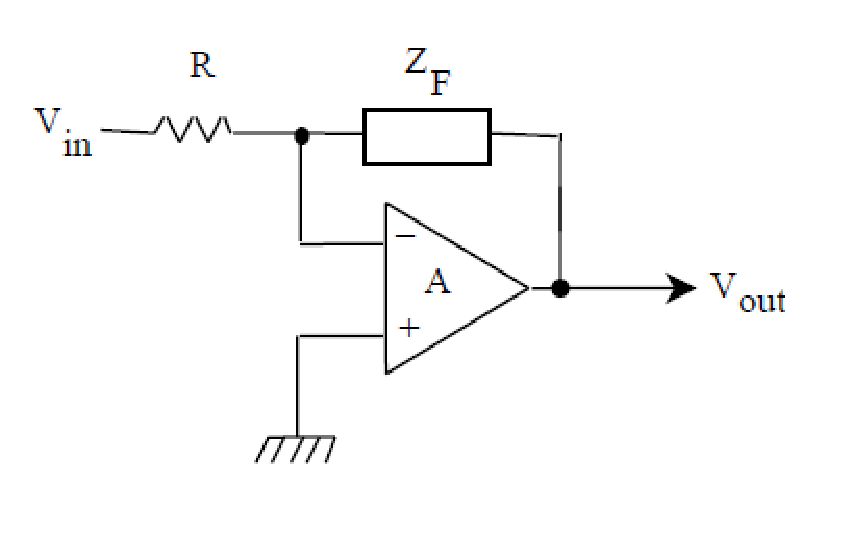
\includegraphics[scale=0.60]{FigLCbandSchem1}
\caption{\textit{The schematic for the LC active bandpass filter. See figure \ref{FigLCbandSchem2} for a schematic of $Z_F$}}
\label{FigLCbandSchem1}
\end{figure}
\begin{figure}[h]
\centering
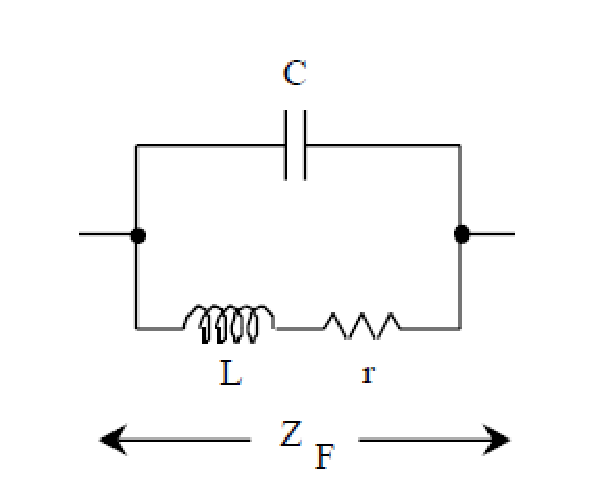
\includegraphics[scale=0.60]{FigLCbandSchem2}
\caption{\textit{The schematic for the $Z_F$ component of the LC active bandpass filter. See figure \ref{FigLCbandSchem1} for a schematic of the rest of the circuit.}}
\label{FigLCbandSchem2}
\end{figure}
We know that the LCR circuit in figure \ref{FigLCbandSchem2} has a resonant frequency $f_0$ given by
\begin{equation}
f_0 = \frac{1}{2\pi}\frac{1}{\sqrt{LC}}
\label{ResFreq}
\end{equation}
So we see that the LC active bandpass filter is an inverting amplifier with gain given by
\begin{equation}
G = -\frac{R_F}{R}
\label{InvGain}
\end{equation}
where $R_F$ in this case is the impedance of the LCR circuit, $Z_F$. So when we have an input frequency of $f_0$ the op-amp produces a very large gain. Given that the gain as a function of $\omega$ as
$$G(\omega) = -\frac{Z_0}{R}\frac{\frac{i\omega}{\omega_0}+\frac{1}{Q}}{-\frac{\omega^2}{\omega_0^2}+\frac{i\omega}{\omega_0Q}+1}$$
Note that $\omega$ is the angular frequency and is related to harmonic frequency by a factor of $2\pi$ or $\omega = 2\pi f$. So $\omega_0$ is given by equation \ref{ResFreq} except for the factor of $2\pi$. $Z_0$ is the characteristic impedance of the LCR circuit. This is given by
\begin{equation}
Z_0 = \sqrt{\frac{L}{C}}
\label{CharImp}
\end{equation}
$Q$ is the quality factor of the circuit which is defined by the resonant frequency,$f_0$, divided by the width of the Bode Plot $3$dB down from $f_0$ this quantity is called $\Delta f$ so
\begin{equation}
Q \equiv \frac{f_0}{\Delta f}
\label{QualDef}
\end{equation}
We can also calculate $Q$ from $Z_0$ through
\begin{equation}
Q = \frac{Z_0}{r}
\label{QualCalc}
\end{equation}
Now if we see that the function $G(\omega)$ at $\omega_0$ becomes
\begin{equation}
G(\omega_0) = -Q\frac{Z_0}{R}
\label{GainPeak}
\end{equation}

\subsection{Oscillator Circuit}
An oscillator circuit is very close to the LC active bandpass filter except we add positive feedback in the form of voltage divider (see figure \ref{FigOscSchem}).
\begin{figure}[h]
\centering
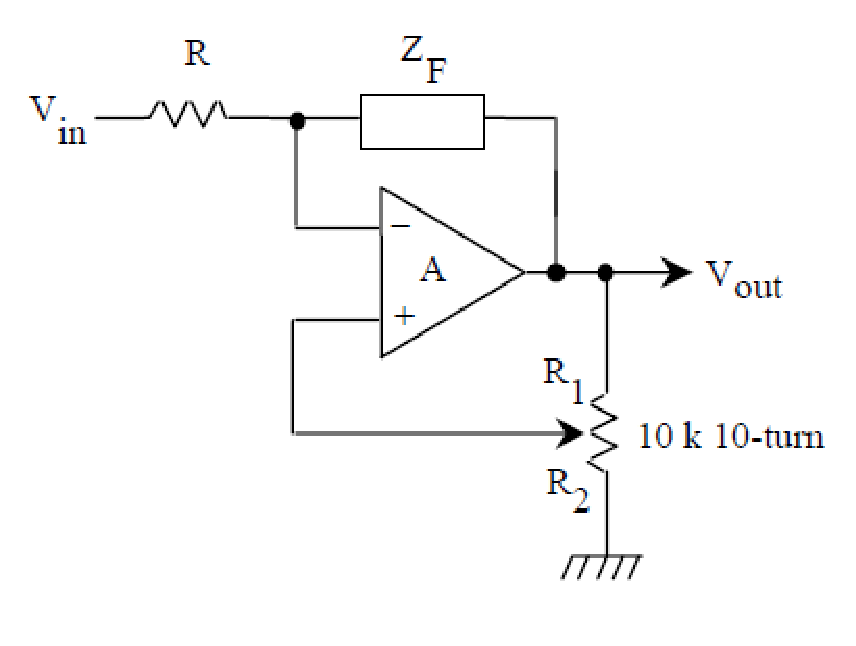
\includegraphics[scale=0.60]{FigOscSchem.eps}
\caption{\textit{The schematic for the oscillator circuit. See figure \ref{FigLCbandSchem2} for a schematic of $Z_F$}}
\label{FigOscSchem}
\end{figure}
We can see that from equation \ref{VoutVpVm} that we can say the gain is given by
$$G = \frac{-A(1-B_-}{1-A(B_+-B_-)}$$
Where $B_+$ and $B_-$ are the voltage divider ratios of the positive and negative inputs. These are given by
$$B_+\frac{R_2}{R_1+R_2};\ B_-\frac{R}{R+R_F}$$ 
This circuit begins to oscillate its output voltage spontaneously when the gain goes to infinity. This is the point where there is a $V_{out}$ even if there is no input voltage. Assuming that $A$ is very large we can say that the gain goes to infinity when $B_+=B_-$. If we assume that the frequency of oscillation is near the resonate frequency we can say that $R_F=Z_0^2/r$ this implies that
$$B_+|_{\textnormal{threshold}} = \left.\frac{R_2}{R_1+R_2}\right|_{\textnormal{threshold}} = \left.\frac{rR}{rR+Z_0^2}\right|_{\textnormal{threshold}}$$
where we can determine the threshold frequency as
\begin{equation}
f_{\textnormal{threshold}} = f_0\sqrt{1-\frac{1}{Q^2}}
\label{ThresFreq}
\end{equation}

\subsection{Schmitt Trigger}
A Schmitt Trigger is a circuit that only has positive feedback. If we remove $Z_F$ from the oscillating circuit we get a Schmitt Trigger (see figure \ref{FigSTrigSchem}).
\begin{figure}[h]
\centering
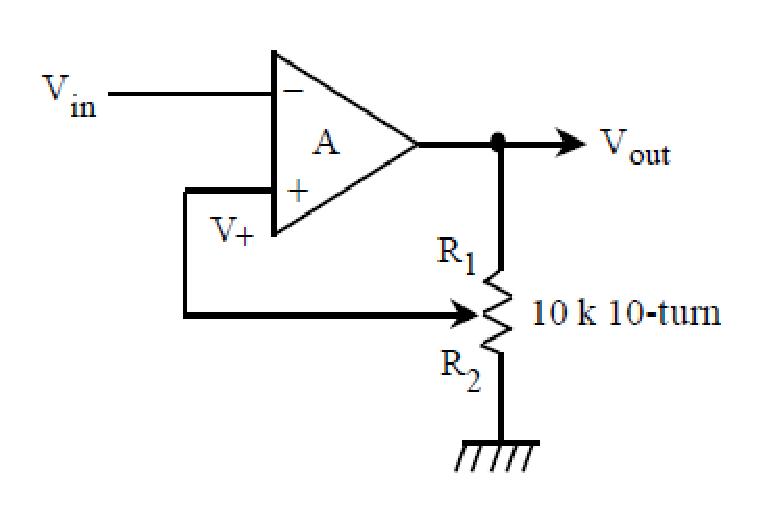
\includegraphics[scale=0.60]{FigSTrigSchem.eps}
\caption{\textit{The schematic for the Schmitt Trigger.}}
\label{FigSTrigSchem}
\end{figure}
This positive feedback loop and it is called a trigger, because once it reaches a voltage above its threshold it will rail the op-amp. This leads to an output voltage that is a square wave when a triangle wave in the input signal. See figure \ref{FigSTrigEXPlot} for an example of this behavior.
\begin{figure}[h]
\centering
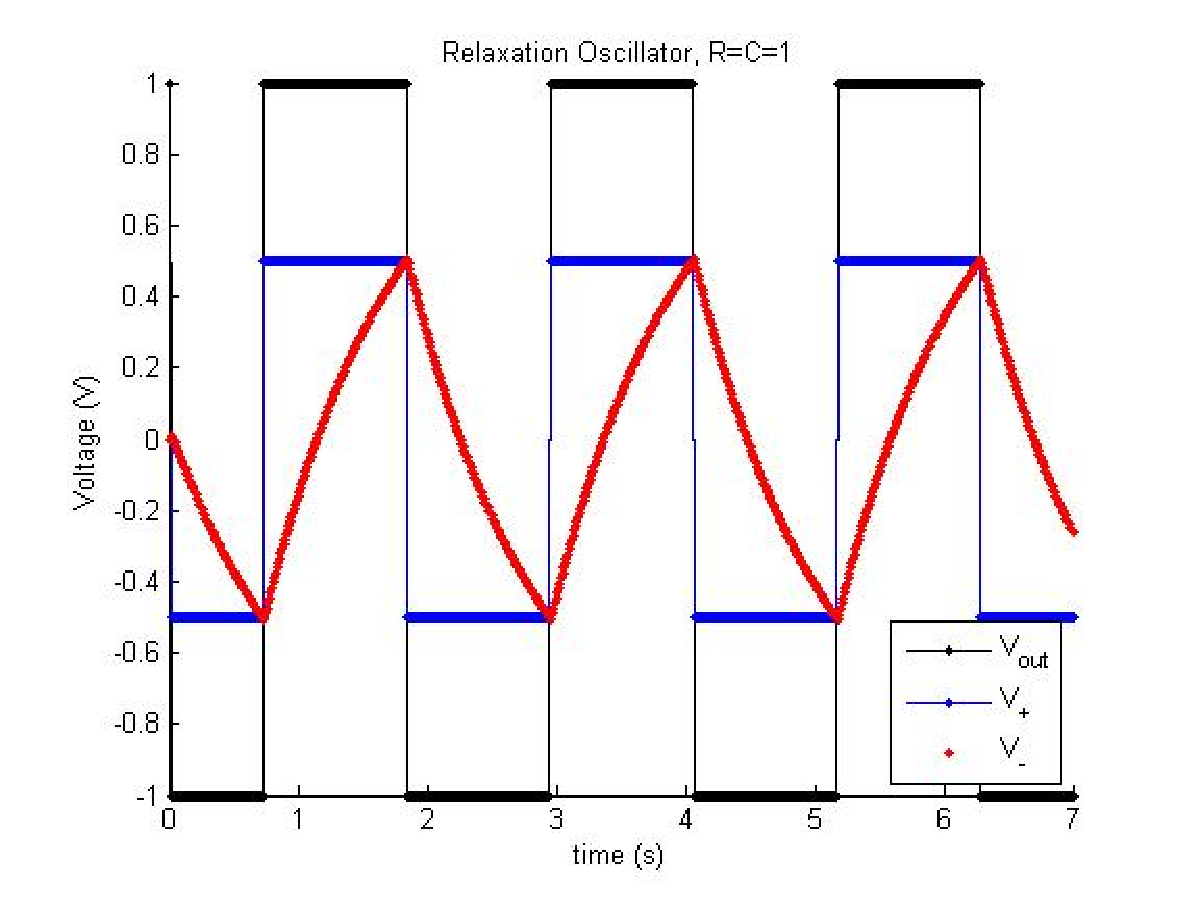
\includegraphics[scale=0.60]{FigSTrigEXPlot.eps}
\caption{\textit{A sample plot of the Schmitt Trigger's response to a input triangle wave.}}
\label{FigSTrigEXPlot}
\end{figure}

\section{Experiment}
We used a function generator for the output voltage signals. We split the output from the function generator to channel one of the oscilloscope and to the circuit. We powered the op-amp using a DC power supply. Note that we set the trigger on the oscilloscope using the function generator. All connections between the devices were made with coaxial cables and banana connections (for the DC power supply).

\subsection{LC Active Bandpass Filter}
To begin we made the circuit in figures \ref{FigLCbandSchem1} and \ref{FigLCbandSchem2}. Where $L=9.44\unit{mH}$, $C=10.26\unit{nF}$, $r=99.1\unit{\Omega}$, and $R=9.86\unit{k\Omega}$. Then we sent an sine wave into the circuit with an amplitude of $1\unit{V_{pp}}$. Next we adjusted the frequency of the input voltage until we found the maximum of the output voltage. The frequency at this point is the resonant frequency, $f_0$, we found that $f_0=16.3\unit{kHz}$. Then we measured the amplitude of the input and output voltages as $V_{in}=1.00\unit{V_{pp}}$ and $V_{out} = 0.748\unit{V_{pp}}$. This gives us our peak gain of the circuit. Which we measured as $G(f_0)=0.748$. 

Next we want to find the quality factor, $Q$. To do this we found where the gain is a $1/\sqrt{2}$ factor of the peak gain, $G(f_0)$. This calculated as $G_{3db} = 0.528$. Note that our input voltage is $1.00\unit{V_{pp}}$, so we adjusted the frequency until the output voltage was $0.528\unit{V_{pp}}$. These frequencies were measured as $f_+=17.5\unit{kHz}$ and $f_-=15.3\unit{kHz}$. This gives us $\Delta f=2.23\unit{kHz}$. Using this value for $\Delta f$ and $f_0=16.3\unit{kHz}$ we us equation \ref{QualDef} to calculate $Q=7.32$. Now if we calculate $Q$ from equation \ref{QualCalc} where $L=9,44\unit{mH}$, $C=10.26\unit{nF}$, and $r=99.1\unit{\Omega}$ we expect that $Q = 9.68$. This is pretty far off of the measured value, but we did not take into account the internal resistance of the inductor $L$.

To take into account the internal resistance of our inductor we solved equation \ref{QualCalc} for $r$ to get
$$r = \frac{Z_0}{Q}$$
and calculated $r$ using $Q=7.32$, $L=9.44\unit{mH}$, and $C=10.26\unit{nF}$. We calculated that $r=131\unit{\Omega}$ for a quality factor of $7.32$. So we see that the internal resistance of the inductor is $32\unit{\Omega}$ so we made changed $r$ to $67.1\unit{\Omega}$ to compensate for the inductor.

We repeated the procedure to find the peak gain and the quality factor. Note that the resonate frequency $f_0$ does not depend on $r$ so it was not changed. We measured the input and output voltage at $f_0$ as $V_{in} = 1.01\unit{V_{pp}}$ and $V_{out}=0.988\unit{V_{pp}}$. So our peak gain is given by $G(f_0) = 0.978$. Next we found the quality factor again using the same method except this time we adjusted the frequency until $V_{out} = 0.698\unit{V_{pp}}$ and we found that $f_+=17.19\unit{kHz}$ and $f_-=15.46\unit{kHz}$. So $\Delta f = 1.73$ and equation \ref{QualDef} yields $Q=9.41$. This is much closer to the expected value of $Q_{expt}=9.68$. Now if we calculate the expected gain for this circuit using equation \ref{GainPeak} and the values we measured for $L$, $C$, and $Q$ we find that we expect that $G(f_0)=0.915$. This expected value is in agreement with our measured value $G(f_0)=0.978$. Note that before we accounted for the inductors internal resistance our gain was very off like our quality factor. 

\subsection{Oscillator Circuit}
First we added positive feedback into the circuit we built for the LC active bandpass filter note that the component values remain unchanged at $L=9.44\unit{mH}$, $C=10.26\unit{nF}$, and $r=67.1\unit{\Omega}$. The positive feedback loop is a voltage divider in the form of a 10-turn $10\unit{k\Omega}$ potentiometer (see figure \ref{FigOscSchem}). Then we removed the resistor $R$ and made the input voltage ground so there was no input signal. Note that our output signal at this point was a flat line at $V_{out} = 0\unit{V_{pp}}$. Next we adjusted the potentiometer until the output voltage was not zero this is the point of spontaneous oscillation. Once we were exactly at this point we removed the potentiometer and measured $R_1 = 5.06\unit{k\Omega}$ and $R_2=5.10\unit{k\Omega}$. So we found that the threshold value of $B_+|_{\textnormal{threshold}} = 0.502$ we expected the value of $B_+|_{\textnormal{threshold}}$ to be one half so the measured result is in agreement with the expected.

We then adjusted the trigger on the oscilloscope so that the waveform will hold still and measured the period of the oscillation using the cursors. We found that one period was $T = 64.0\unit{\mu s}$. Taking the inverse of this we found the frequency at the threshold is $f_{\textnormal{threshold}} = 15.9\unit{kHz}$. Using equation \ref{ThresFreq} where $Q=9.41$ and $f_0 = 16.3\unit{kHz}$ we expect that $f_{\textnormal{threshold}} = 16.1\unit{kHz}$. Note that these values are in agreement.

Next we measured the amplitude of the output voltage to differing divider ratios $B_+$. We did this by adjusting the potentiometer. To measure the output voltage we had to set the trigger on the oscilloscope to keep the waveform from moving constantly. To measure $B_+$ we measured $R_1$ and the total resistance of the potentiometer as $R_P = 10.14\unit{k\Omega}$ using the digital multimeter. We then calculated $R_2$ and $B_+$ using these values. See table \ref{TabOsc} for the data and the plot in figure \ref{PlotOsc}.
\begin{table}[h]
\centering
\begin{tabular}{cccc}
$R_1$			&$R_2$			&$B_+$		&$V_{out}$\\
\hline
$6.09\unit{k\Omega}$	&$4.05\unit{k\Omega}$	&$0.399$	&$0.00\unit{V_{pp}}$\\
$5.59\unit{k\Omega}$	&$4.55\unit{k\Omega}$	&$0.449$	&$0.00\unit{V_{pp}}$\\
$5.09\unit{k\Omega}$	&$5.05\unit{k\Omega}$	&$0.498$	&$1.11\unit{V_{pp}}$\\
$4.82\unit{k\Omega}$	&$5.32\unit{k\Omega}$	&$0.525$	&$6.48\unit{V_{pp}}$\\
$4.57\unit{k\Omega}$	&$5.57\unit{k\Omega}$	&$0.549$	&$22.9\unit{V_{pp}}$\\
$4.51\unit{k\Omega}$	&$5.63\unit{k\Omega}$	&$0.555$	&$27.3\unit{V_{pp}}$\\
\end{tabular}
\caption{\textit{A table of the output voltage vs a changing divider ratio $B_+$. Note that we measured $R_1$ and the total resistance of the potentiometer as $10.14\unit{k\Omega}$ using these values we calculated $R_2$ and $B_+$.}}
\label{TabOsc}
\end{table}
\begin{figure}[h]
\centering
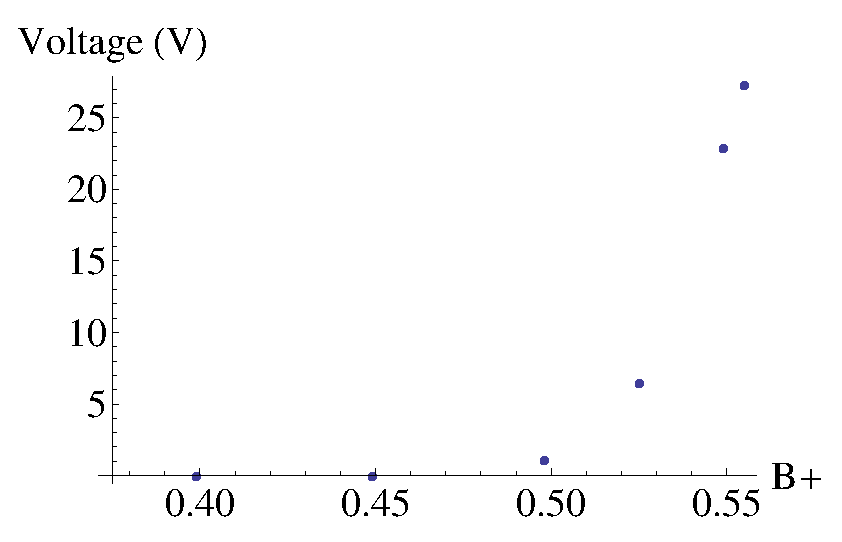
\includegraphics[scale=0.70]{PlotOsc.eps}
\caption{\textit{A plot of $B_+$ versus $V_{out}$ note the exponential rise in the output voltage. See table \ref{TabOsc} for the data in the plot.}}
\label{PlotOsc}
\end{figure}

\subsection{Schmitt Trigger}
We removed the LCR component from our circuit to create a Schmitt Trigger in figure \ref{FigSTrigSchem}. We then sent a triangle wave into the circuit with an amplitude of $2\unit{V_{pp}}$. We adjusted the potentiometer until the op-amp railed. The waveforms from the oscilloscope are attached. Note that the peaks of the triangle wave are on a different phase then the square wave produced.

\section{Conclusion}
This lab has demonstrated the effects of stray capacitance and inductance on an op-amp. Namely when we have positive feedback. We see that even with no input voltage we can get a spontaneous oscillation when we reach the right feedback voltage. The effect on the output signal can is hard to predict since the spontaneous oscillations are not easily defined functions, but if we are just looking for a binary response of above or below the threshold the spontaneous effect can be very useful.


\end{document}

